\chapter{Setup and execution}
This chapter will discuss the setup that is used to produce and detect the $\si{\tera\hertz}$-electric field.
As well as the method that is used to achieve a time-resolved measurement of the $\si{\tera\hertz}$ pulse.

\section{Setup}
\label{sec:setup}
To produce $\si{\tera\hertz}$ radiation the setup as shown in Figure \ref{fig:setup} is used.
A Ti-sapphire laser is used to produce the necessary laser radiation.
It produces a pulsed laser beam with a power of around $\SI{6.9}{\W}$, with a frequency of $\SI{1000}{\Hz}$.
However because the laser feeds into several setups only a fraction of the initial power reaches each setup.
This setup receives between $\SI{579}{\milli\W}$ and $\SI{291}{\milli\W}$ depending on the configurations of the other setups. 
The incoming laser with a pulse length of $\SI{100}{\femto\second}$ is split into a pump and a probe laser.
The pump beam receives $90\%$ of the initial laser beam power, and the probe beam the remaining $10\%$.
The pump beam passes through a chopper which modulates the laser to a frequency of $\SI{280}{\hertz}$.
This way the lock-in Amplifier that is used for the measurement can be triggered on that frequency.
After the chopper, a delay stage is placed.
With this, the pump beam path length can be altered.
This allows a time-resolved detection of the $\si{\tera\hertz}$ pulse, a detailed description can be found in section \ref{sec:time_domain}.
To focus the beam on the crystal a lens with a focal length of $\SI{40}{\centi\meter}$ is placed $\SI{15}{\centi\meter}$ infront of the crystal.
This distance is just enough to focus all the beam power on the whole crystal surface.
Ultimately the beam is hits the emitter crystal.
Depending on the measurement a zinc telluride (ZnTe) or a gallium phosphite (GaP) crystal is used.
\\
With this part of the setup done $\si{\tera\hertz}$ radiation can already be produced, just the detection is still missing.
\\\\
To detect the $\si{\tera\hertz}$ radiation it first needs to be seperated from the laser light that is transmitted by the emitter crystal.
In this setup a silicon wafer blocks the transmitted laser beam and transmits the $\si{\tera\hertz}$ radiation, which is generated by the emitter crystal.
Two parabolic mirrors focus the $\si{\tera\hertz}$ beam onto the detection crystal.
As detection unit a $\SI{1}{\milli\meter}$ ZnTe crystal is used.
To place the detection crystal right at the focus of the parabolic mirror, a light source can be used to reflected into the mirror.
The detection crystal can then be moved to the focus of that light cone.
The same methode can be used to place the emitter crystal at the corrcet distance from the first mirror.
\\\\
The probe beam, whose power is reduced by an optical density filter, passes through the back of the second parabolic mirror, which has a small hole in it.
From there it hits the detection crystal at roughly the same position as the pump $\si{\tera\hertz}$ beam.
To make sure that this is the case, the emitter crystal and the silicon wafer can be removed and a strong optical density filter is placed into the pump beam.
The filter is necessary because the pump laser beam would damage the parabolic mirrors otherwise.
Now the parabolic mirrors reflect the actual laser pump beam onto the detection crystal.
With an infrared viewing camera it is than possible to see if the pump laser and probe laser actually overlap.
If that is the case the pump $\si{\tera\hertz}$ beam should be atleast roughly at the same position as the pump laser beam.
Which means the $\si{\tera\hertz}$ pump beam also overlaps with the probe beam.
After the aligment of pump and probe beam on the detector crystal, the emitter crystal is placed back into the setup aswell as the silicon wafer.
With this the first part of the detection unit is done, the $\si{\tera\hertz}$ radiation should now change the polarization of the probebeam.
\\\\
The next step is to measure the change of polarization.
As described in section \ref{sec:eos}, the polarization of the probe beam is change depending on the $\si{\tera\hertz}$-electric field.
After the change in polarization, the probe beam passes through a quarter-wave plate \ref{sec:qwp}, which changes the linear polarization of the beam to an elliptic polarization.
The quarter-wave plate is also used to balance the signal while there is now $\si{\tera\hertz}$ electric field.
This way the photodiodes have an equal output if there is no change in polarization from the detector crystal.
The beam is then split into its horizontal and vertical polarization components by a Wollaston prism, which is further explained in subsection \ref{sec:wollaston}
The two separate beams are passed into photodiodes.
\\\\
Depending on the polarization of the probe beam after the detection crystal the intensity of the probe beams after the Wollaston prism change.
The signal of the photodiodes $A$ and $B$ is passed into a lock-in Amplifier, which calculates the difference between both signals $A-B$.
The bigger the difference $A-B$ the stronger the $\si{\tera\hertz}$-electric field in the detection crystal.
\\\\
With the setup now done the signal has to be optimized.
To do this the stage is moved to the position of the strongest signal.
The changes that are being made to the setup should now increase the height of the peak or lower the noise in comparission to the peak signal.
As shown in subsection \ref{sec:znte} the orientation of the ZnTe is of great importance.
That is why the first step should be to rotated the emitter crystal, to the point were the $<001>$ cyrstal direction is parallel to the polarization of the pump beam.
After the correct rotation is found the process is repeated for the detection crystal.
Now the pump laser beam position on the emitter crystal needs to be adjusted.
For this the laser mirror before the crystal is slowing being rotated until the signal is at its greatest stregnth.
Now the parabolic mirrors should be adjusted by moving their position and orientation slightly.
The signal can also be increased by rotating the detection crystal, so that the probe beam does not hit it perpendicular.
The best results were achieved with an angle of $\SI{40}{\degree}$.
Finaly the overlap of $\si{\tera\hertz}$ pump beam and laser probe beam on the detection crystal should be corrected.


\FloatBarrier
\subsection{Quater-wave plate}
\label{sec:qwp}
To balance the two photodiodes, a quarter-wave plate is used.
This component changes the polarization of the incoming electric field into a circular or elliptical polarization, depending on its orientation.
It is also possible to not change the polarization at all if the quarter-wave plate and electric field are aligned in a certain way.
The quarter-wave plate introduces a phase shift of $\symup{exp}(i\frac{\pi}{2}) = i$ into the electric field of one polarization component of the wave.
This way the incoming wave $\vec{E}$, that consist of a horizontally polarized component $E_\text{h}\vec{h}$ and a vertically polarized component $E_\text{v}\vec{v}$, can be written as
\begin{equation}
    \vec{E} = (E_\text{v}\vec{v} + E_\text{h}\vec{h})\symup{e}^{i(kx-\omega t)}
\end{equation}
and changes after the quarter wave plate to 
\begin{equation}
    \vec{E} = (E_\text{v}\vec{v} + i E_\text{h}\vec{h})\symup{e}^{i(kx-\omega t)}
\end{equation}
if the phase shift is induced along the horizontal polarized axis it will result into an elliptical polarization as seen in the lower part of figure \ref{fig:qwp}.
It works the same way if the phase shift is induced at the vertical axis.
If now the electric field strengths in both polarization directions are the same $E_\text{v} = E_\text{h} = E$ the result of the phase shift is a circularly polarized wave
\begin{equation}
    \vec{E} = E(\vec{v} + i\vec{h})\symup{e}^{i(kx-\omega t)} \, .
\end{equation}
By rotating the quarter-wave plate it is then possible to induce the phaseshift to both polarization components with different extend.
For the right balancing, the quarter-wave plate changes the polarization of the probe beam to a circular one, if there is no $\si{\tera\hertz}$ signal and to an elliptical, if there is a signal.
\begin{figure}
    \centering
    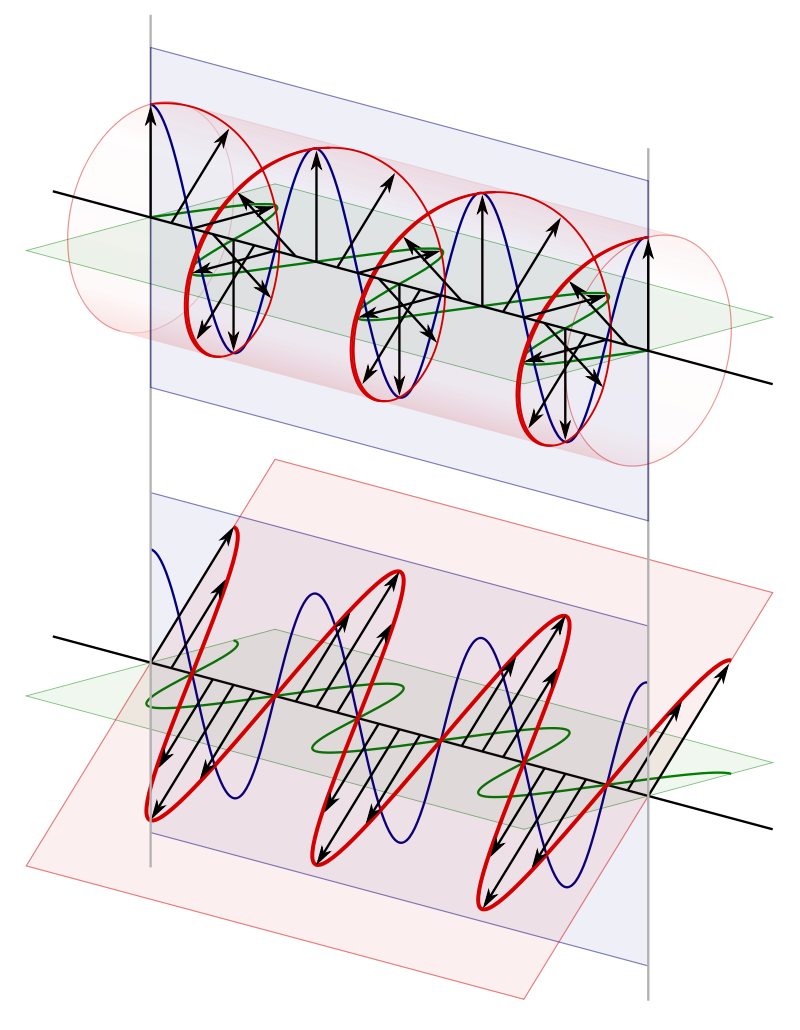
\includegraphics[width=0.4\textwidth]{refferenced_pic/qwp.png}
    \caption{Depending on the initial polarization the quarter-wave plate changes the polarization of the electric field to a circular (upper picture) or elliptical polarization (lower picture).
    The picture is taken from source \cite{qwp}.}
    \label{fig:qwp}
\end{figure}
\FloatBarrier
\subsection{Wollaston prism}
\label{sec:wollaston}
The probe beam polarization, after the detector crystal, carries all the information about the $\si{\tera\hertz}$-electric field strength.
Because it is not possible to measure the polarization of the probe beam directly, it is necessary to split the probe beam into its two polarization components.
This happens with a Wollaston prism, shown in figure \ref{fig:wollaston}.
It consists of two prisms that are glued together.
The light that passes through the prism now refracts at the point where the two prsims touch.
From the Fresnel equations, it is possible to derive, that depending on the polarization of the light it gets refracted differently.
In case of the Wollaston prism, this means that the beam splits into a horizontally and a vertically polarized beam, with an angle of about $\SI{20}{\degree}$.
It is then easy to detect the intensity of both beams to derive the change in polarization that occurred at the detector crystal. 
\begin{figure}
    \centering
    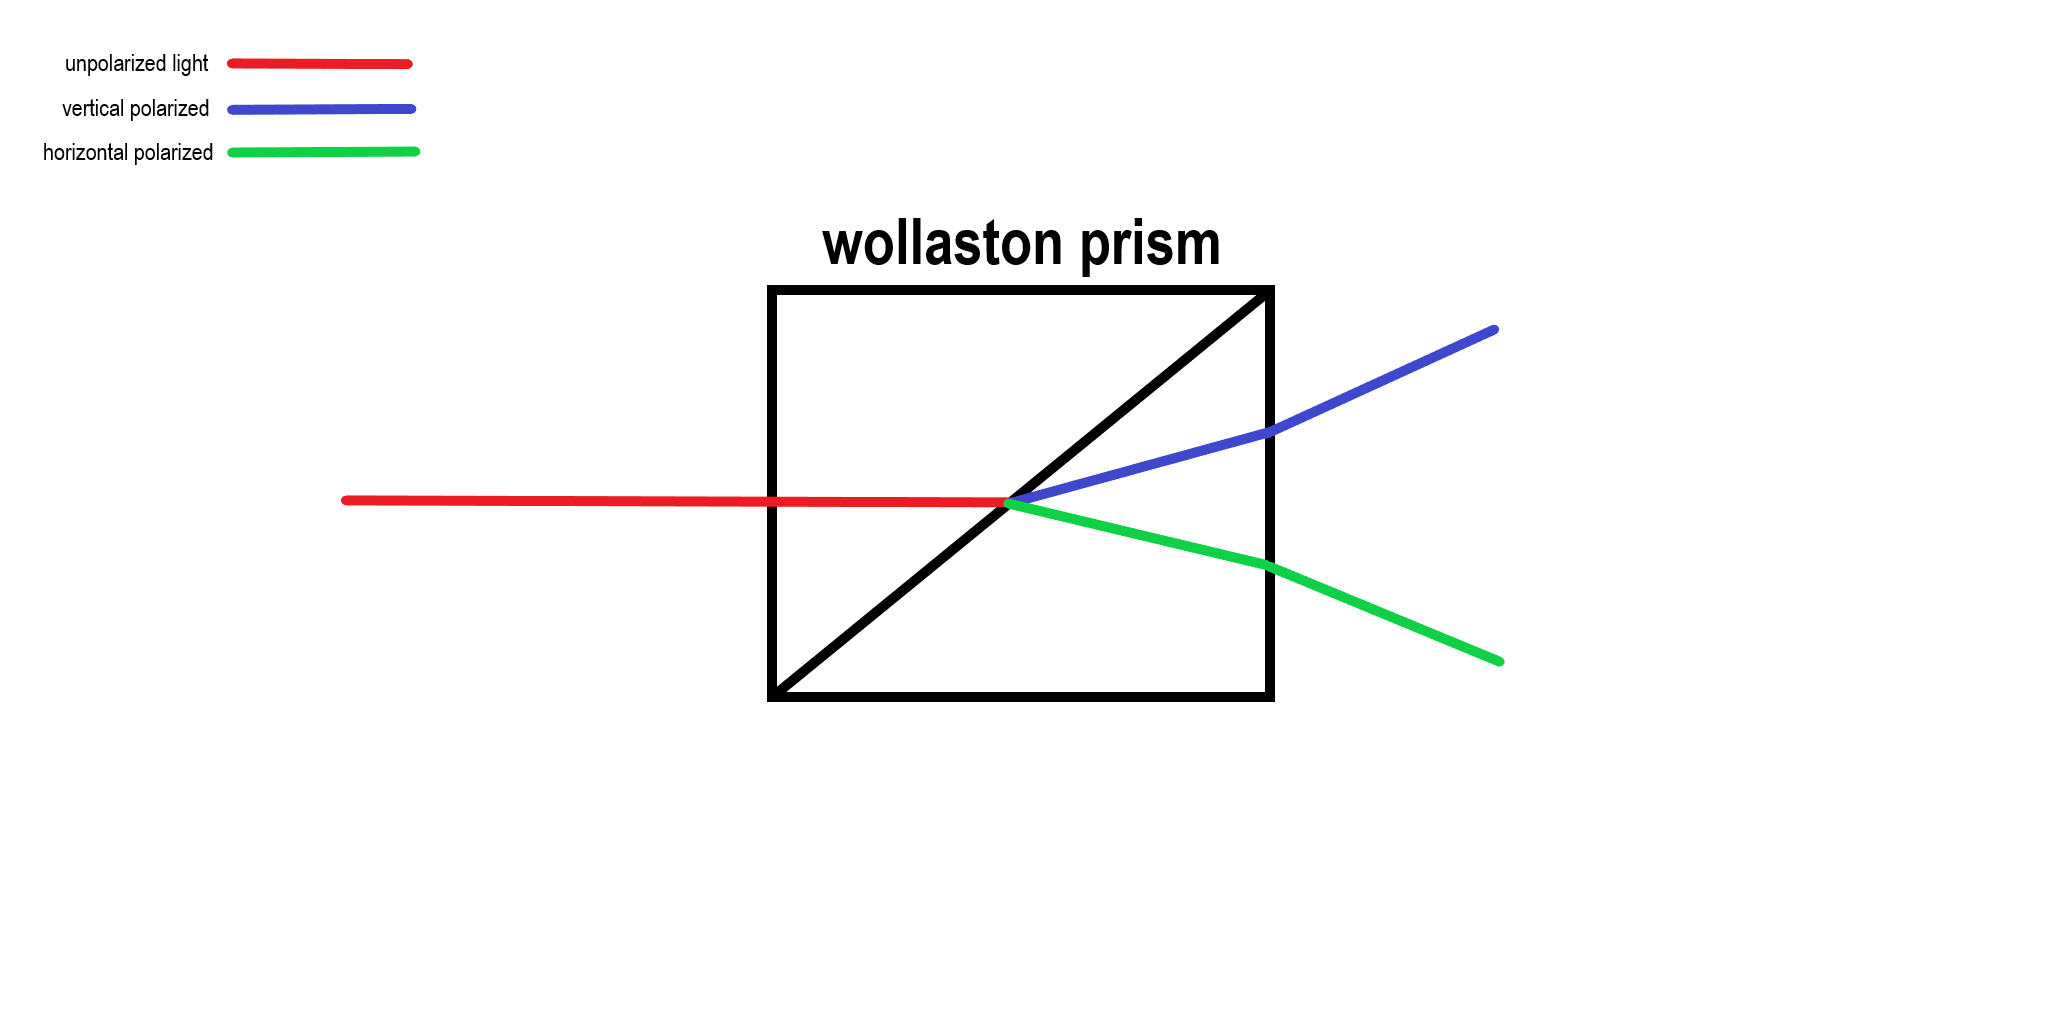
\includegraphics[width=0.7\textwidth]{refferenced_pic/wollaston.png}
    \caption{The picture shows a Wollaston prism through which an unpolarized beam passes.
    This beam refracts inside the prism which splits into two beams with perpendicular polarization.
    The two beams then leave the prism with an angle between them.}
    \label{fig:wollaston}
\end{figure}
\section{Time-resolved THz spectroscopy}
\label{sec:time_domain}
To achieve a time-resolved measurement of the $\si{\tera\hertz}$-pulse a delay stage is built into the setup.
With the delay stage, the path length of the pump beam can be changed.
This way a time delay between the pump pulse and the probe pulse is achieved.
Because the velocity of electromagnetic radiation in air is roughly the same as in a vacuum, the vacuum speed can be used to calculate the time delay   
\begin{equation}
    \Delta t = \frac{\Delta s}{c}
\end{equation}
with $c$ as the speed of light, and $\Delta s$ the difference in the beam path legnth.
The time-resolved measurement now works by taking one measurement at delay stage position $s_1$, which corresponds to $t_1$.
Then the stage is moved to position $s_2$ this lengthens or shortens the beam path of the pump beam.
At stage position $s_2$ a new measurement is taken which corresponds to time $t_2$.
Now there is a time delay $\Delta t_{1-2} = t_1 - t_2$ between the two measurements.
This process is repeated until the whole $\si{\tera\hertz}$-pulse is probed.
For this the delay stage has to be moved roughly $\SI{4}{\milli\meter}$.
To get a good resolution $1000$ measurements with a distance of $\SI{0.004}{\milli\meter}$ between them are taken.
This distance corresponds to a time resolution of $\SI{13.34}{\femto\second}$.

\section{Execution}
This section describes how the measurements were taken. 
It will be discussed what changes to the setup in figure \ref{fig:setup} are being made to achieve the wanted results.
\\\\
Before any measurements are taken the photodiodes have to be balanced.
For this a chopper is placed inside the probe beam, which modulates its frequency to $\SI{388}{\hertz}$.
The lock-in amplifier gets triggered on that frequency, while its inputs are the $A$ and $B$ values of the two photodiodes.
It is necessary to move the stage to a point where $\si{\tera\hertz}$-pulse and probe pulse do not overlap so that the polarization of the probe beam is not changed by the detector crystal.
Now the quarter-wave plate is being rotated until the output of both photodiodes $A-B = 0$.
Usually, the difference is never zero, because the photodiode output suffers from noise.
To acount for the noise the quarter-wave plate is rotated until the average of $A-B$ over a small time period is zero.
If that is the case the probe beam is circularly polarized after the quarter-wave plate, while it is not affected by the $\si{\tera\hertz}$ signal.
\\\\

\subsection{Fluence measurements}
The goal of the fluence measurements is to determine the effect of different pump fluences on the $\si{\tera\hertz}$ production.
For it is necessary to change the power of the pump beam before it hits the emitter crystal.
For that different density filters are placed inside the beam path.
All the filters that were used can be seen in table \ref{tab:filters}.
The filters are placed inside a mount right after the chopper.
After the placement, the pump power is measured behind the filter.
Then the power meter is removed so that the pump hits the emitter crystal.
Now a short measurement with a low time resolution is taken to roughly determine the position of the signal peak.
After the peak position is found a time-resolved measurement, as described in section \ref{sec:time_domain}, of the pulse is taken.
For this, the stage is moved to its starting position at about $\SI{1}{\milli\meter}$ before the signal peak.
It stops $\SI{3}{\milli\meter}$ after the peak.
These positions are chosen to only scan the pulse and the oscillations that occur after the pulse.
It should also be said that reflections inside the emitter and the detector crystals cause a so-called pre- and post-pulse.
These are unwanted byproducts of the initial pulse and will interfere with later calculations.
This makes it important to only measure the initial pulse but not the pre- and post-pulse.
After the measurement, the filter is swapped out with another one and the process is started over until all fluences are measured.

\subsection{Electric field measurements}
To determine the electric field of the $\si{\tera\hertz}$ radiation it is necessary to measure the output of the photodiodes $A$ and $B$ separately as well as their difference $A-B$.
Because just the maximum field strength is of particular interest just the greatest $A-B$ value is necessary to measure.
For this, the delay stage is moved into the peak of the pulse, which is the position of the greatest $A-B$ value and a measurement of the difference is taken.
This process has to be repeated for all pump power values that are wanted.
After all the differences are measured, $A$ and $B$ are measured separately.
The delay stage is moved to a position where there is no $\si{\tera\hertz}$ signal.
At this position, the input of the lock-in amplifier is changed to just one of the outputs of the photodiodes, either $A$ or $B$.
Because the sum $A+B$ is not affected by the $\si{\tera\hertz}$ electric field, it can be used to norm every difference.
So the separately measured values of $A$ and $B$ have to be measured just once.
After $A-B$ and $A$ and $B$ are measured the electric field can be calculated.





\subsection{Transmission measurements}
